\subsection{Study Area}
El área metropolitana de Monterrey (MMA) se localiza en la parte noreste de México, con una población de 4.7 millones de personas distribuidas 18 municipios que en total abarcan 7,657 m$^2$ \cite{inegi2015}. Las principales actividades económicas se encuentran comercio, servicios inmobiliarios, construcción y fabricación de maquinaria y equipo que se realizan 213 grupos industriales, la mayoría con sede en el MMA. El MMA está rodeado por la Sierra Madre Oriental, el Cerro de la Silla, el Cerro de las Mitras y el Cerro del Topo Chico (figura \ref{fig:map}), las cuales crean una barrera física natural para la circulación del viento que impiden el desalojo del aire contaminado hacia el exterior de la zona.\cite{proaire2008}
\begin{figure}[H]
    \centering
    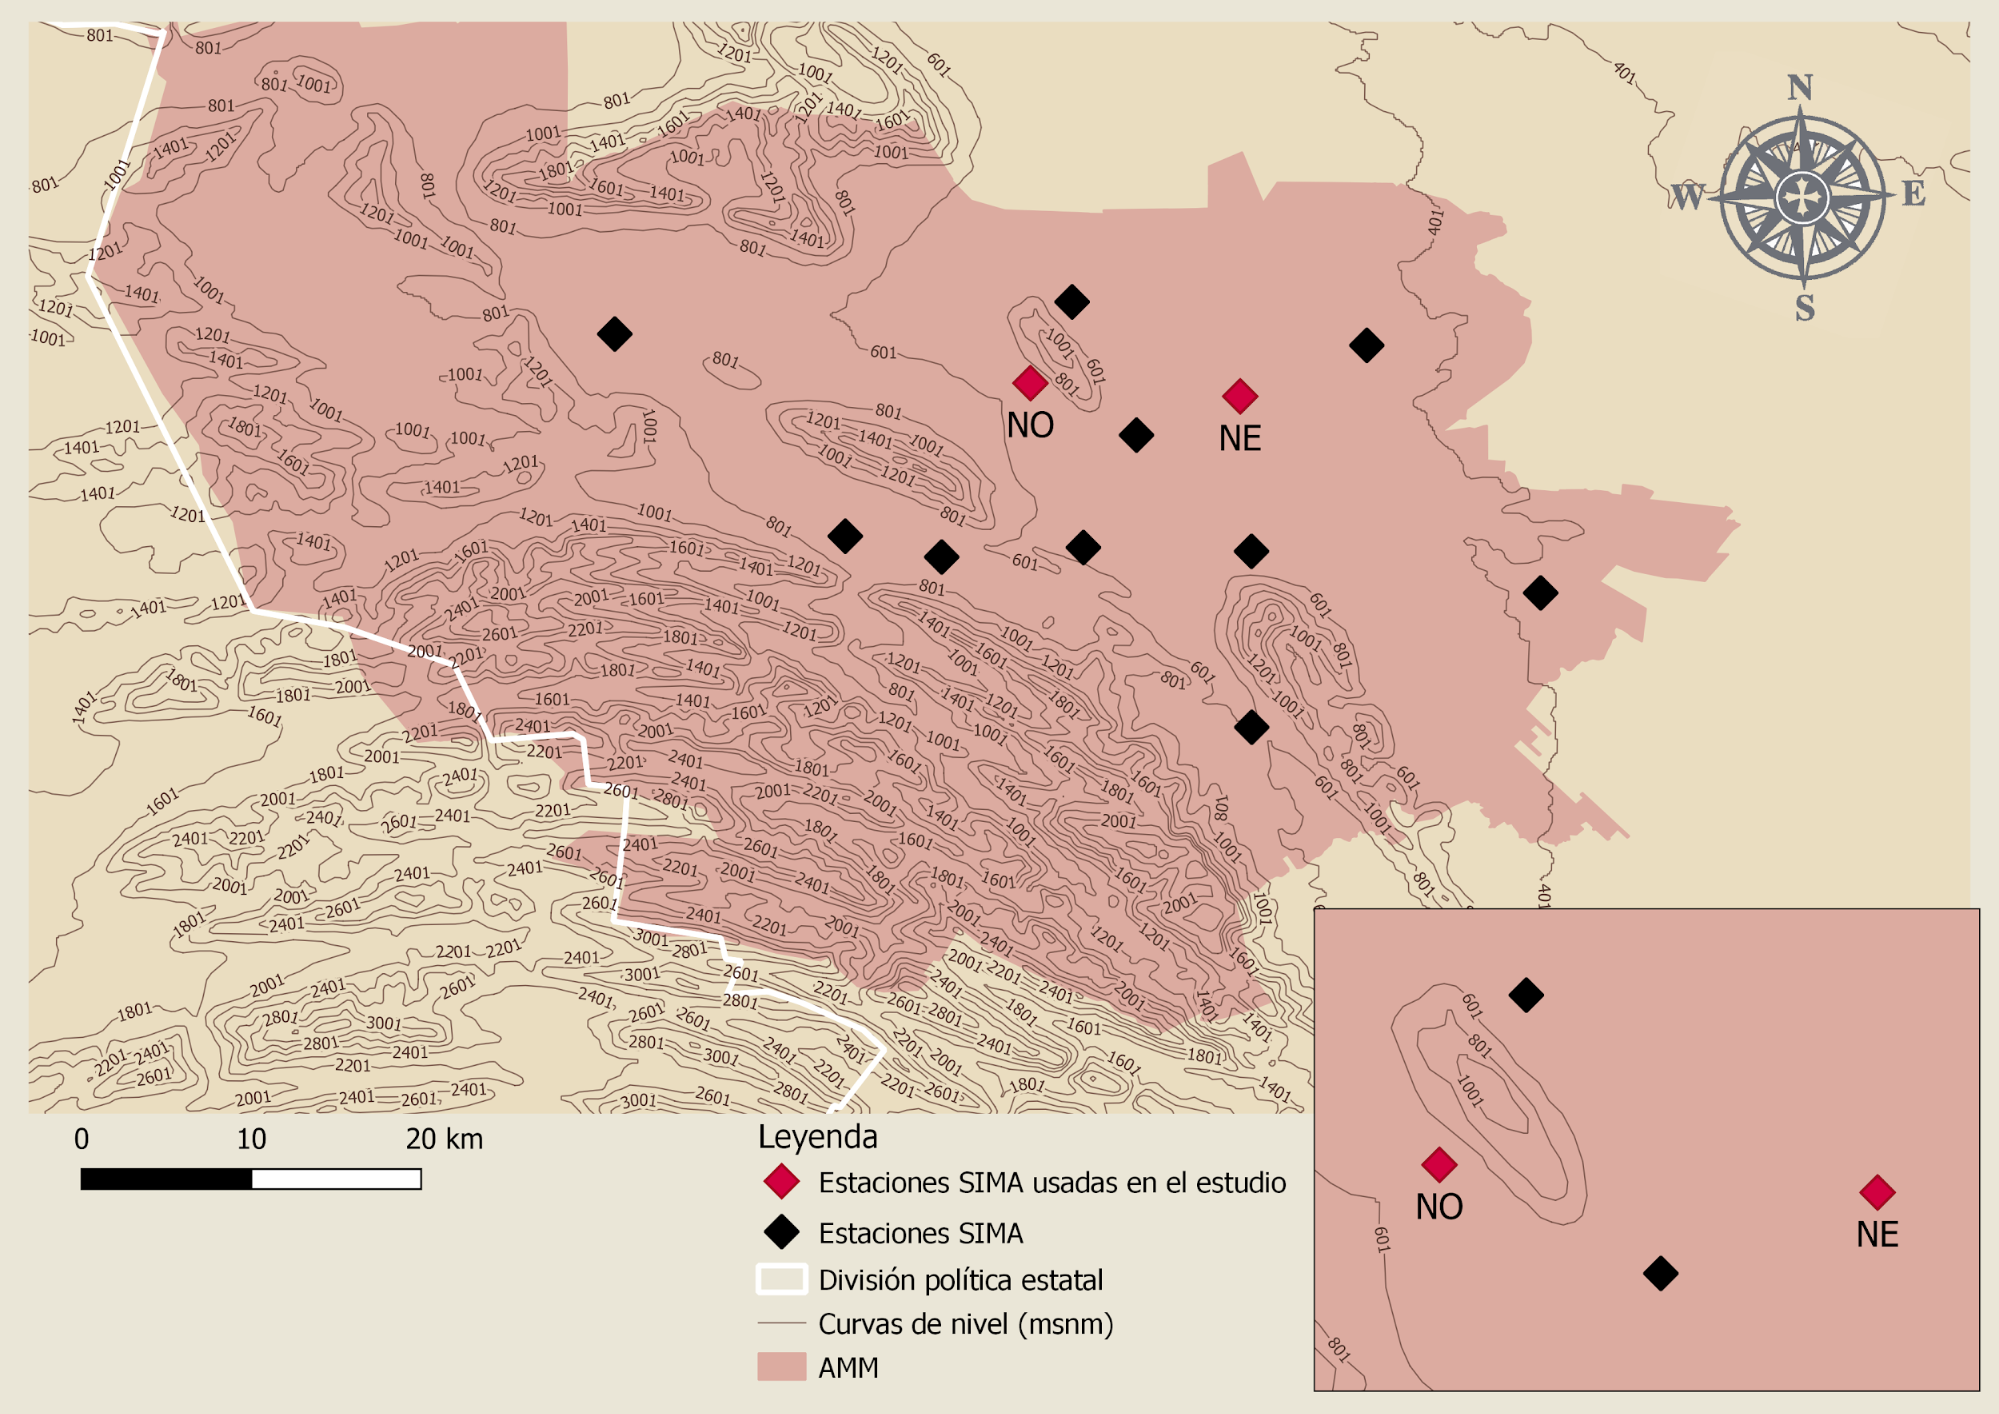
\includegraphics[scale=0.2]{images/map.png}
    \caption{Área Metropolitana de Monterrey con sus principales cerros y sierras.}
    \label{fig:map}
\end{figure}
El Sistema Integral de Monitoreo Ambiental (SIMA) inició sus operaciones en el año 1992 con cinco estaciones de monitoreo. En el año 2017 el número de estaciones en operación aumentó a 13, siendo las estaciones Universidad, Serena y Cadereyta las últimas instaladas en este año \cite{simapage}. La localización geográfica y clasificación de las estaciones de monitoreo se encuentran en la Tabla \ref{table:stations_loc}. La clasificación de las estaciones corresponde con la descripción dada por la Secretaría de Medio Ambiente y Recursos Natuales (SEMARNAT). \cite{proaire2016}
\begin{table}[H]
    \begin{tabular}{llcccc} \hline
    Station name   & Code       & Altitude (MSL) & Latitude   & Longitude    & Operating since \\ \hline
    Obispado       & CE         & 560              & 25.67 & -100.34 & Sep/1992     \\
    Escobedo       & N          & 528              & 25.80 & -100.34 & Dec/2009     \\
    Universidad    & N2         & 520              & 25.73 & -100.31 & Oct/2017     \\
    San Nicolás    & NE         & 476              & 25.75 & -100.26 & Sep/1992     \\
    Apodaca        & NE2        & 432              & 25.78 & -100.19 & Jun/2011     \\
    San Bernabé    & NW         & 571              & 25.76 & -100.37 & Sep/1992     \\
    García         & NW2        & 716              & 25.78 & -100.59 & July/2009    \\
    Serena         & S          & 630              & 25.57 & -100.25 & Oct/2017     \\
    Pastora        & SE         & 492              & 25.67 & -100.25 & Sep/1992     \\
    Juárez         & SE2        & 387              & 25.65 & -100.10 & Nov/2012     \\
    Cadereyta      & SE3        & 340              & 25.36 & -100.00 & Aug/2017     \\
    Santa Catarina & SW         & 694              & 25.68 & -100.46 & Sep/1992     \\
    San Pedro      & SW2        & 636              & 25.66 & -100.41 & Feb/2014     \\ \hline
    \end{tabular}
\caption{}
\label{table:stations_loc}
\end{table}
\subsection{Meteorology, solar irradiance and PM\textsubscript{10} measurements}
En la Tabla \ref{table:measurements_SIMA} se muestra el porcentaje de mediciones anuales disponibles en cada estación de la red del SIMA. En rojo se representan las estaciones que tienen un porcentaje menor a 75\%, ya que con esto se considera que las mediciones son insuficientes para una estadística anual \cite{molina2019}.
\begin{table}[H]
    \changefontsizes{9pt}
    \begin{tabular}{lcccccccccccc}
        \hline
        \multicolumn{1}{c}{}                       & \multicolumn{2}{c}{2015} & \multicolumn{2}{c}{2016} & \multicolumn{2}{c}{2017} & \multicolumn{2}{c}{2018} & \multicolumn{2}{c}{2019}                            & \multicolumn{2}{c}{2020}                                                                                                                                                                                                    \\ \cline{2-13}
        \multicolumn{1}{c}{\multirow{-2}{*}{Code}} & PM\textsubscript{10}     & SR                       & PM\textsubscript{10}     & SR                       & PM\textsubscript{10}                                & SR                                                  & PM\textsubscript{10} & SR   & PM\textsubscript{10} & SR                                                  & PM\textsubscript{10}                                & SR   \\ \hline
        CE                                         & 94.6                     & 95.8                     & 97.0                     & 97.7                     & 96.8                                                & 98.2                                                & 94.8                 & 99.1 & 95.1                 & 94.5                                                & 92.8                                                & 96.5 \\
        N                                          & 76.8                     & 98.8                     & 98.1                     & 97.9                     & 93.0                                                & 96.6                                                & 94.1                 & 97.6 & 96.3                 & 99.9                                                & \cellcolor[HTML]{CB0000}{\color[HTML]{FFFFFF} 73.7} & 84.3 \\
        N2                                         & -                        & -                        & -                        & -                        & \cellcolor[HTML]{CB0000}{\color[HTML]{FFFFFF} 20.9} & \cellcolor[HTML]{CB0000}{\color[HTML]{FFFFFF} 25.1} & 94.3                 & 98.6 & 94.4                 & 98.8                                                & 92.3                                                & 99.1 \\
        NE                                         & 93.9                     & 83.9                     & 98.3                     & 96.9                     & 98.1                                                & 99.2                                                & 97.4                 & 99.8 & 98.5                 & 99.5                                                & 92.8                                                & 89.3 \\
        NE2                                        & 89.9                     & 98.3                     & 93.7                     & 99.9                     & 96.3                                                & 99.8                                                & 96.1                 & 99.4 & 94.5                 & 99.1                                                & 91.1                                                & 98.1 \\
        NW                                         & 95.3                     & 99.3                     & 98.1                     & 94.9                     & 98.5                                                & 99.7                                                & 94.9                 & 99.5 & 90.9                 & 94.4                                                & 96.5                                                & 98.7 \\
        NW2                                        & 83.8                     & 97.7                     & 84.3                     & 88.5                     & 95.7                                                & 99.0                                                & 96.6                 & 99.5 & 95.8                 & 98.2                                                & 96.4                                                & 99.4 \\
        S                                          & -                        & -                        & -                        & -                        & \cellcolor[HTML]{CB0000}{\color[HTML]{FFFFFF} 22.8} & \cellcolor[HTML]{CB0000}{\color[HTML]{FFFFFF} 23.7} & 92.9                 & 99.4 & 96.7                 & 99.6                                                & 94.8                                                & 99.9 \\
        SE                                         & 92.8                     & 98.6                     & 97.2                     & 99.0                     & 98.4                                                & 99.1                                                & 94.3                 & 98.5 & 95.9                 & 98.4                                                & 94.1                                                & 99.1 \\
        SE2                                        & 95.9                     & 99.6                     & 99.1                     & 100.0                    & 95.7                                                & 97.4                                                & 92.4                 & 99.6 & 95.8                 & \cellcolor[HTML]{CB0000}{\color[HTML]{FFFFFF} 64.2} & 90.3                                                & 99.7 \\
        SE3                                        & -                        & -                        & -                        & -                        & \cellcolor[HTML]{CB0000}{\color[HTML]{FFFFFF} 37.1} & \cellcolor[HTML]{CB0000}{\color[HTML]{FFFFFF} 38.6} & 95.1                 & 99.1 & 98.3                 & 99.8                                                & 94.1                                                & 99.7 \\
        SW                                         & 92.3                     & 97.2                     & 96.9                     & 98.7                     & 97.9                                                & 99.6                                                & 92.6                 & 99.2 & 97.9                 & 99.6                                                & 97.0                                                & 99.6 \\
        SW2                                        & 88.4                     & 96.5                     & 96.8                     & 98.6                     & 93.6                                                & 98.1                                                & 95.1                 & 99.5 & 96.7                 & 99.7                                                & 90.8                                                & 99.9 \\ \hline
    \end{tabular}
    \caption{Porcentaje anual de las mediciones de PM\textsubscript{10} e irradiancia solar de las estacion del SIMA en el periodo 2015-2020.}
    \label{table:measurements_SIMA}
\end{table}
Se seleccionaron las estaciones de San Nicolás y San Bernabé ya que el radiómetro instalado es el Pyranometer Model 095. Se seleccionaron los días de cielo despejado, el criterio de clasificación consiste en grafícar la irradiancia solar diaria y si forma una función gaussiana (figura \ref{fig:clear_days}) entonces ese día contiene hubo cielo despejado.
\begin{figure}[H]
    \centering
    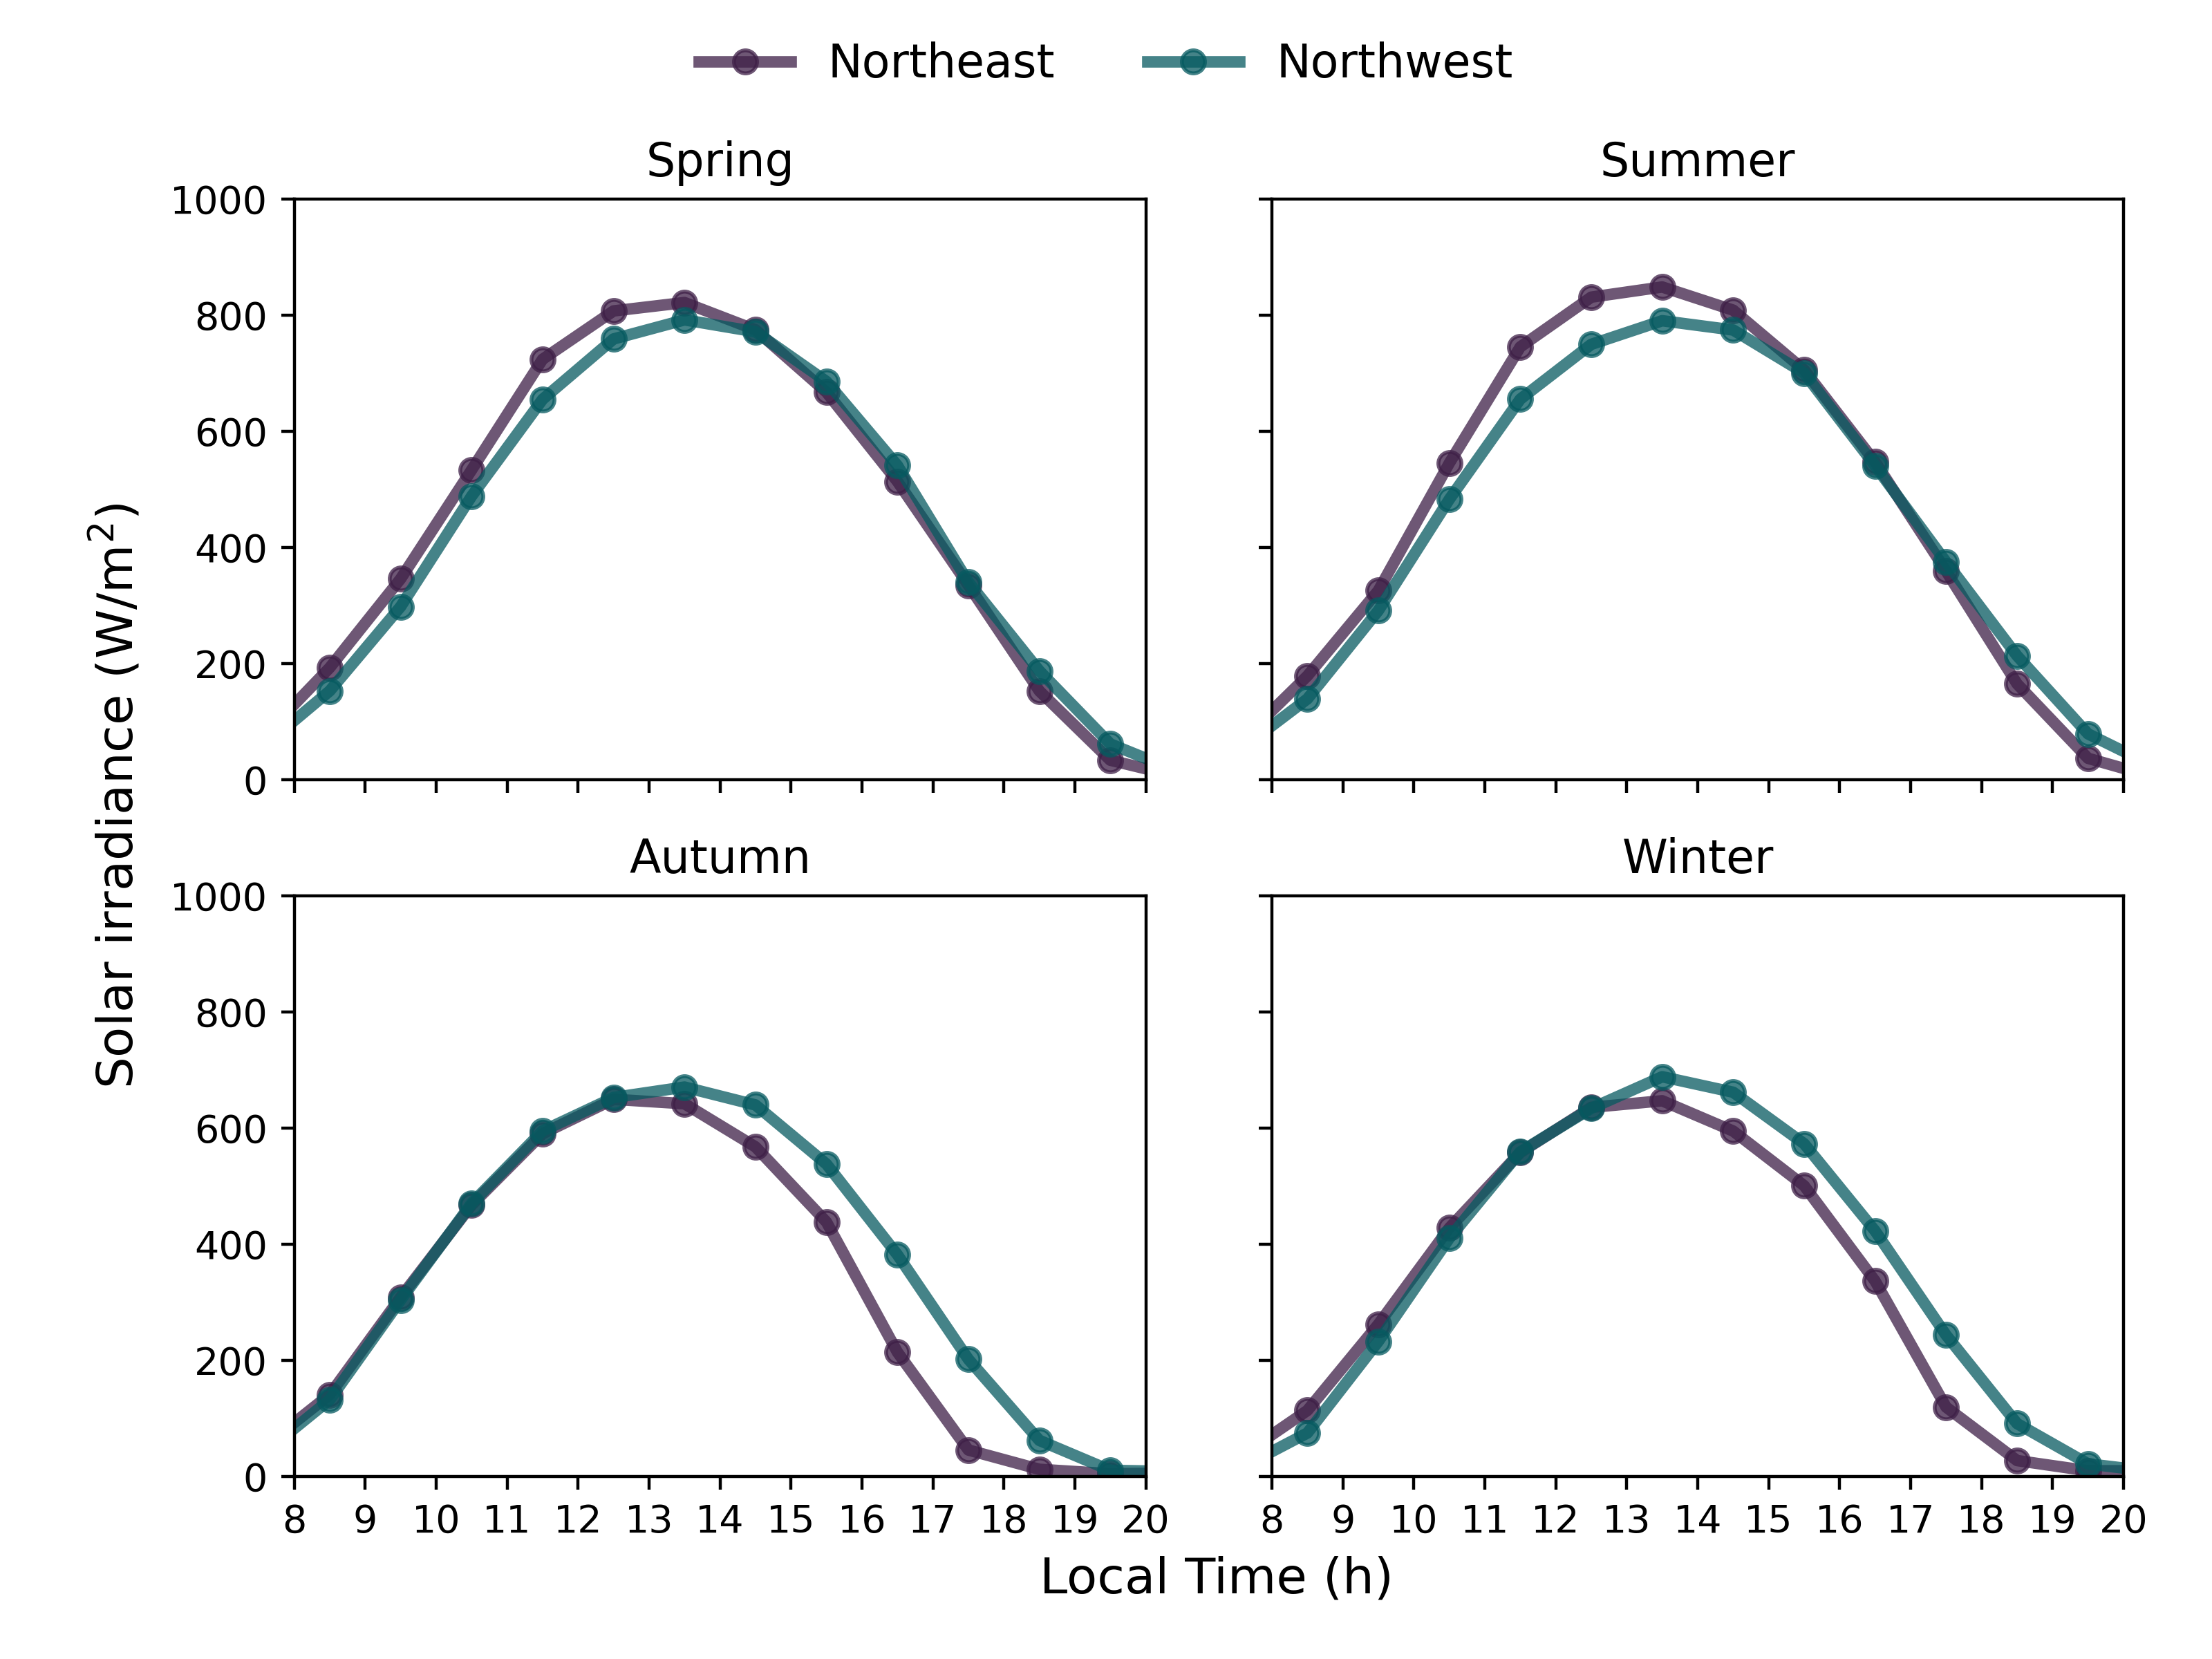
\includegraphics[scale=0.5]{images/Clear_days.png}
    \caption{Promedio de la irradiancia solar para cada epoca del año en las estaciones San Nicolás y San Bernabé.}
    \label{fig:clear_days}
\end{figure}
En cada estación de monitoreo no necesariamente miden sin nubosidad al mismo tiempo, esto provoca que la selección de días de cielo despejado no sea la misma en todas las estaciones.